\documentclass[12pt,oneside]{fithesis2}
\newenvironment{changemargin}[2]{%
\begin{list}{}{%
\setlength{\topsep}{0pt}%
\setlength{\leftmargin}{#1}%
\setlength{\rightmargin}{#2}%
\setlength{\listparindent}{\parindent}%
\setlength{\itemindent}{\parindent}%
\setlength{\parsep}{\parskip}%
}%
\item[]}{\end{list}}
\usepackage[english]{babel}
\usepackage[utf8]{inputenc}
\usepackage[T1]{fontenc}
\usepackage[backend=bibtex, style=numeric]{biblatex}
\addbibresource{bib-db.bib}
\usepackage{fixltx2e}
\usepackage[plainpages=false,pdfpagelabels,unicode]{hyperref}
\usepackage{indentfirst}
\usepackage{setspace}
\usepackage{listings}
\usepackage{lscape}
\usepackage{enumitem}
\usepackage{tabularx}
\usepackage{graphics}
\usepackage{epstopdf}
\usepackage{float}
\usepackage{mathtools}
\thesistitle{Real-time collaboration in Komodo} 
\thesislogo{fi-logo.mf}
\thesissubtitle{Diploma thesis}
\thesisstudent{Bc. Matúš Makový} 
\thesiswoman{false} 
\thesislang{en} 
\thesisfaculty{fi}
\thesisyear{Spring 2015}
\thesisadvisor{RNDr. Filip Nguyen} 
\setstretch{1.2}
\begin{document}
\FrontMatter
\ThesisTitlePage
\begin{ThesisDeclaration}
\DeclarationText
\AdvisorName
\end{ThesisDeclaration}
\begin{ThesisThanks}
I would like to thank RNDr. Filip Nguyen for the patience, guidance and advice during my work on this thesis. I would also like to thank Barry LaFond and Paul Richardson from Komodo Team for the answers provided to my questions during my work on the practical part of the thesis.
\end{ThesisThanks}
\begin{ThesisAbstract}
This thesis deals with techniques for real-time collaboration and with recommending of the best technique for Komodo software. Techniques analyzed in the first part of this thesis are Operational Transformation, Differential Synchronization and Commutative Replicated Data Types. These techniques are described and explained. In the first part, there is also a comparison of these techniques according to specified criteria.
\par The second part deals with a recommendation of the best technique suitable for Komodo software, which is the new upcoming version of tooling for Red Hat JBoss Data Virtualization. The most suitable technique is Commutative Replicated Data Types. This part also recommends algorithms for implementation and describes recommendations and requirements for the implementation of this technique in the Java programming language.
\end{ThesisAbstract}
\begin{ThesisKeyWords}
Operational Transformation, Differential Synchronization, Commutative Replicated Data Types, real-time, collaboration, Komodo, Java, CRDTs
\end{ThesisKeyWords}
\tableofcontents 
\MainMatter
\chapter{Introduction} 
Many software solutions enable people to create new things in a better and faster way. In most cases the resulting product is so complex that one person is not enough for successful and fast creation. Creators try to collaborate to achieve a common goal. Among other opportunities and possibilities are collaboration and sharing the greatest benefits of the Internet. \par
We can identify two types of collaboration over the Internet, non-real-time collaboration and real-time collaboration. 
\par In the beginning, as the Internet didn't have such capacity, people tried to use it just for sharing their drafts of work and sending them to each other; this type of collaboration is called non-real-time. In non-real-time collaboration, users would work on separate copies of a project and then need to merge their changes into one final project. In other words, they had to find differences between their drafts and reflect them to each other's versions. It doesn't offer as much flexibility as real-time collaboration and also it had many limitations, for example two people could not edit the same file in a project without having to resolve conflicts manually when they tried to merge their work with a collaborator's version. An example of non-real-time collaboration would be Revision Control (Git, SVN).\par
With the development of the Internet came a reasonable solution called real-time collaboration. Using this principle, the author can see what his collaborator is doing in real-time and manual synchronization or manual conflict resolution is not necessary. Information technologies take care of this synchronization and provide conflict resolution for users.
\par In the theoretical part of this thesis, principles of real-time collaboration are dealt with and descriptions are provided of three of the techniques used to implement real-time collaboration in software over the Internet. In the following chapter, comparison criteria are set in order to compare these techniques in general. 
\par The practical part of this thesis presents a brief description of Red Hat JBoss Data Virtualization and Teiid Designer and also presents Komodo software as a new version of Teiid Designer. Komodo should use real-time collaboration in its upcoming release. We present the requirements of this software on technique, recommend the best one for this authoring software and set the requirements and recommendations on implementation in the Java programming language.

\chapter{Real-time Collaboration}
This chapter covers the basic overview of collaboration in general and a description of real-time collaboration along with a description of difficulties with its implementation over the Internet. The Last sections of this chapter describe three techniques used for implementation over the Internet and its properties. Techniques described in this chapter are: Operational Transformation, Differential Synchronization and Commutative replicated data types.
\section{Basic overview}
Collaboration, as defined by an English dictionary, is an act of working with another or others on a joint project. Authoring Systems in IT that support collaboration are called Groupware. \par "Groupware systems are computer-based systems that support \\two or more users engaged in a common task, and that provide an interface to a shared environment. These systems frequently require fine-granularity sharing of data and fast response times." \cite{Ellis} \par There are many techniques used in groupware systems that are not suitable for real-time collaboration, for example, Locking or Single Active Participant technique. Fundamental principle of Locking and Single Active Participant is to lock data when it is being modified by someone. This principle is adopted for example by Microsoft, when users try to edit a shared document. \par When using real-time collaboration, authoring software creates an illusion that users are working on one common copy of a document online. There is no requirement to commit changes to some kind of shared repository and no need for a user to resolve conflicts. Changes should be reflected and saved immediately. Examples of real-time collaborative editors that we recognize today are Google Docs, Etherpad and the already terminated Google Wave. A software engineer has different options for the implementation of real-time collaboration in a software solution. \par Requirements for good technique are: 
\begin{itemize}
\item speed,
\item latency toleration,
\item low data transfer,
\item consistency maintenance,
\item and good conflict resolution.
\end{itemize}
\par The speed requirement means that changes made on one side of the collaboration process need to be reflected to the other sides as soon as possible and vice versa. Changes should be sent to other collaborators as soon as they are done. If a collaboration technique is fast enough it is much easier to satisfy other requirements. A fast enough technique is able to maintain good consistency. "The system’s response time is the time necessary for the actions of one user to be reflected by their own interface; the notification time is the time necessary for one user’s actions to be propagated to the remaining users’ interfaces." \cite{Ellis} Response time and notification time should be as short as possible.  \par One of the problems of real-time collaborative editing could be network latency. The implemented technique should be able to tolerate the latency of Internet connections, because collaborators could be in very distinct parts of the world. It should be able to reconstruct the right order of operations because data sent over the Internet doesn't necessary arrive in the right order and the order of the operations is very important to maintain consistency.\par A low data transfer requirement is also very important. The different sides of the collaboration should send the smallest amount of data possible. Transferred data should only describe changes that have been done on one side of the collaboration; it is not necessary to transfer the whole project. The less data that it is necessary to transfer, the faster the whole protocol can be.  \par Consistency maintenance is necessary for the success. It has to be ensured, that users on both sides are looking at the same version of a document regardless of the number and complexity of operations being done on both sides of the collaboration. A lack of consistency could cause other problems and chaos in the differing document versions. According to \cite{Vidot} there are three problems encountered when trying to achieve consistency maintenance and they correspond to the properties of the CCI consistency model proposed in \cite{Sun}
\begin{enumerate}
\item \textbf{Causality Preservation} - operation \(O_{1}\) causally precedes operation \(O_{2}\) if \(O_{1}\) occurred locally before \(O_{2}\). The problem is to execute operations in the right order on all sites.
\item \textbf{User Intention Preservation} - the technique must preserve the user's intention in the context of the state in which the operation was executed. This problem strongly relates to the conflict resolution requirement and occurs when it is not possible to determine if \(O_{x}\) causally precedes \(O_{y}\) or \(O_{y}\) causally precedes \(O_{x}\).
\item \textbf{Convergence} - when the same operations have been applied on every site, the documents are identical.
\end{enumerate}
\par Because operations can be done at any time in real-time collaboration, there the problem of concurrency arises. This means, that changes can happen at the same time and in the same sections of a project. A good conflict resolution requirement is required because of concurrency. Implementation techniques have to be able to identify and resolve a conflict when users are editing the same part of the project. \par The concurrency control algorithms are separated into two classes: pessimistic and optimistic. \par "Pessimistic algorithms require communication with other sites or with a central coordinator before making a change to data." \cite{Jupiter} One example of a pessimistic algorithm can be the aforementioned Locking or Single Active Participant technique. \par "Optimistic concurrency control, on the other hand, requires no communication before applying changes locally. The party making a change applies it immediately, then informs the other parties of the action. If more than one participant makes a change at the same time, a conflict resolution algorithm creates compensating changes to move everyone to the same final state." \cite{Jupiter} \par This implies that optimistic algorithms are a better solution for the Internet, because the latency can not be guaranteed. 
\section{Operational Transformation}
\par Operational Transformation (OT) is an optimistic concurrency control algorithm used for real-time collaborative editing over the Internet. 
\par It was first introduced in the paper Concurrency Control in Groupware Systems \cite{Ellis} in 1989, together with the Distributed Operational Transformation (dOPT) Algorithm. "The algorithm has a number of properties which make it suitable for groupware. First, operations are performed immediately on their originating site, thus responsiveness is good. Secondly, locks are not necessary so all data remains accessible to group members. Finally, the algorithm is fully distributed, and resilient to site failure..."\cite{Ellis} \par This first algorithm was able to process only plain text. Later some problems with correctness were discovered and resolved in following works. Over the years many other algorithms implementing OT have been published. Algorithms used today are also able to process XML and other formats. \par OT was used also in the Jupiter Collaboration System in 1995 \cite{Jupiter}. Jupiter's two-way algorithm is derived from the dOPT algorithm used by Grove in \cite{Ellis}. This algorithm is one of the improvements of dOPT. \par Today Google is one of the most common implementers of this protocol. The main application was in the Google Wave project, which is now terminated although Operational Transformation is also found in the Google Docs project. According to \cite{Spiewak} Google is one of the biggest innovators of this approach an its biggest contribution is the idea of operation composition, which is described later in this section. \par The approaches differ also in the architecture, dOPT doesn't involve server in its architecture, but recent algorithms use a central server that maintains its version of the document, coordinates the communication and broadcasts operations.
\par This section explains the basic principles of Operational Transformation using the Google version of the control algorithm. It introduces some improvements added by Google and then point out the differences between the presented version and other versions like dOTP, Jupiter and TIPS. 
\par The basic idea is that data are replicated on every machine and the only information that is sent over the Internet are the operations. Data replication ensures good responsiveness in high latency environments. Among Wave's additions to OT are also annotations. "An annotation is some meta-data associated with an item range, i.e., a start position and an end position. This is particularly useful for describing text formatting and spelling suggestions, as it does not unnecessarily complicate the underlying structured document format." \cite{Google} \par The main building block of this approach, as the name suggests, is an operation. Here are the operations defined for use in Google Wave \cite{Google}:
\begin{itemize}
\item retain() - move cursor
\item insertCharacters() - inserts texts
\item insertElementStart() - inserts starting tag
\item insertElementEnd() - inserts end tag
\item deleteCharacters() - deletes text
\item deleteElementStart() - deletes starting tag
\item deleteElementEnd() - deletes ending tag
\item replaceAttributes() - replaces attributes in tag
\item updateAttributes() - updates attributes in tag
\item annotationBoundary() - describes changes in annotations
\end{itemize}
\par The operation is executed locally and then sent over the network to the server or to other peers, to execute the operation on their version of the document. Every object that can be changed in the document has its index for identification. Google Wave uses XML as the format for storing information so a character in text and also a starting and terminating tag in XML structure are considered to be objects for Operational Transformation.  (characters of tags are not considered to be objects). 
\par The second major part of this technique is a transformation function that transforms operations. Operations which are sent over the network and received by the server cannot be executed directly on the server's version of the document, because the index of the desired element could be different in the local copy and in the server copy of the document and this can cause inconsistency and violation of User Intention Preservation. See Figure~\ref{fig:ot} with an example for better explanation. \par For the purpose of this example, we will assume that we have one client that sends operations done on his local copy and a server that receives operations from all peers and maintains a server version of the document. 
\begin{figure}[H]
\caption{Example - Operational Transformation}
\label{fig:ot}
\centering
\vspace{5mm}
\includegraphics{op1}
\end{figure}
Both of them start with the text 'TAX' in their document. The pointer starts at index 0 and the operation retain() shifts the pointer by a number of indexes given as a parameter. The client wants to add the character 'E' so he executes the operations:
\vspace{3mm}
\begin{verbatim}
retain(3);
insertCharacters('E');
\end{verbatim} 
\vspace{3mm}
In the meantime the server received an operation from another peer that has inserted the character 'S', so server executes the operations:
\vspace{3mm} 
\begin{verbatim}
retain(3);
insertCharacters('S');
\end{verbatim}
\vspace{3mm}
The server and client exchange the operations. The different order and difference in indexes on both sides of the collaboration result in an inconsistent document state. The string in the first document is 'TAXSE' and the string in the second document is 'TAXES'.  In order to preserve the user's intention and to attain the correct result we have to transform these operations. The correct result after inserting the letters 'E' and 'S' should be 'TAXES'. The server has the correct version of the document, but the client doesn't so we have to transform the operation sent by the server to look like this:
\vspace{3mm}
\begin{verbatim}
retain(4);
insertCharacters('S');
\end{verbatim}
\vspace{3mm}
This transformation was helpful, but it is not enough. Now the client's operation retains 3 characters, inserts a new character and leaves the cursor in front of the last letter while the server's operation retains 4 characters inserts a character and leaves the cursor behind the whole word. The client and server should end up in the same state so it is also necessary to transform the client's operation: 
\vspace{3mm}
\begin{verbatim}
retain(3);
insertCharacters('E');
retain(1);
\end{verbatim}
\vspace{3mm}
After this change the result of applying operations on both sides will be correct.\par More generally, if we have two operations \(O_{1}\) and  \(O_{2}\) we need a transformation function \textit{transform}, such that: 
\begin{center}
\(transform(O_{1},O_{2}) = (O'_{1},O'_{2}) \quad where \quad O'_{2} \circ O_{1} \equiv O'_{1} \circ O_{2} \) 
\end{center}
In other words, the function takes two operations and transforms them against each other and the output of the function are two transformed operations, such that, if we have the same strings on both sides a we apply \( O_{1} \) and \(O'_{2}\) on one side, and \( O_{2} \) and  \( O'_{1} \) on the other side, the resulting string is the same. 
\par Operational Transformation systems can also support undo functions, but the complexity of the algorithm rises. "If an OT system is to support particular functionality, then it must be able to support certain transformation properties. For group editing and consistency maintenance, the system must support a transformation function known as Inclusion Transformation (IT). For group undo, where the effect of a previously executed operation is un-done at all sites, and all operations executed after it are all re-transformed, the system must support another transformation function known as Exclusion Transformation(ET). Inclusion Transformation transforms operation \( O_{A} \) against another operation \( O_{B} \) in such a way that the impact of \( O_{B} \) is effectively included. Exclusion Transformation transforms operation \( O_{A} \) against another operation \( O_{B} \) in such a way that the impact of \( O_{B} \) s effectively excluded." \cite{Leung} 
\par The problem described in Figure~\ref{fig:ot} could also be visualized as a "diamond problem"; see Figure~\ref{fig:diamond1}
\begin{figure}[H]
\caption{Diamond Problem - 1}
\label{fig:diamond1}
\centering
\vspace{5mm}
\includegraphics{diamond1}
\end{figure}
Operations completed by a peer take the document to the left side and the operations completed on a server take the document to the right side. Each node in the diamond diagram represents the number of operations done by a client and server in a particular state. 
\par As for the example, the correct scenario would be that the peer and server exchange their operations, each one computes its transformation and applies the transformed operation on their versions of the documents.
\par The problem presented by this example is actually the only one that Operational Transformation is capable of solving. A complicated situation occurs when the sides of the collaboration diverge by more than one step. 
\begin{figure}[H]
\caption{Diamond problem - 2}
\label{fig:diamond2}
\centering
\vspace{5mm}
\includegraphics{diamond2}
\end{figure}
This example is used in \cite{Spiewak}. On the server side, transformation for operations \(a,c\) has to be computed, and the server applies operation \(a'\) on its version of the document. The remaining operation \(c'\) has to be preserved for the next transformation. During the next step the server must use \(b\) and \(c'\) as an input and computes \(b'\) that can be applied on its version of the document. The server's document is in the desired state. 
\par On the client side, \(c\) has to be transformed against two operations to get to the desired state. For two operations it is not a big problem, but as the number of operations could very quickly increase, because Operational Transformation is an optimistic technique, so it could potentially take a long time to process. One of the advantages of the Google Wave Operational Transformation is that it is able to compose the operations if they are compatible. This Composer is able to validate operations to make sure that they are compatible and compose them. One of the criteria for compatibility is that operations must span the same number of indexes.  If operations \(a\) and \(b\) are composed into operation \(d\), the transformation function can take operations \(d,c\) and produce operation \(c''\) that can be applied to the peer's document and the document is in the desired state. 
\par This example is still simple. It does not point out some necessary parts of Operational Transformation. The importance of the preservation of operation \(c'\) was obvious from the diagram, but without the diagram it is hard to determine what operation the server or client should preserve. In order to make it easier, metadata about the parent state of the operation is added. Every operation has an identifier of the state in which it was executed. Google Wave uses a scalar version number, but Daniel Spiewak in \cite{Spiewak} suggests to use a hash of the documents contents. 
\par Having the parentage information, the server is able to determine that the parent state of operation \(b\) is not in the server's history and it has to derive a new operation that would take the document to the state after the application of operations \(a\) and \(c\) which will be the parent state of \(b\). This operation is \(c'\). This deriving of operation \(c'\) is called bridging.
\par With this new feature there comes a new problem. In order to derive the operation \(c'\) the server also has to preserve operation \(a\). This could be a scalability problem in an environment with many clients editing the same document, since server has to potentially preserve this data for every client. This is resolved by transferring all the responsibility to the client and buffering the operations on the client's side. 
\par The client can only send operations that come from the state in the server's history and can also send only one operation to the server and has to wait for the acknowledgment of the operation. All following operations are preserved in the buffer on the client's side. One of the advantages of buffering operations is that if these operations are compatible, they can be composed using the Composer. When the server acknowledges the first operation, the client can send the next operation. This way the client can predict the server's path and only send operations that are on the server's path. Also it is much more complicated for the server to track every client, but it is generally much easier for the client to track only one server. This way the server solves only the one-step diamond problem presented in the first example.
\par Daniel Spiewak in the article Understanding and Applying Operational Transformation \cite{Spiewak} describes some other improvements of Operational Transformation by Google Wave. For example, when the client receives operation from the server and has some operations in the buffer, he can transform the whole buffer against this operation in order to accelerate the process on his site and also to ensure that operations in the buffer have a parent state in the server's history.
\par This technique is obviously not so easy to implement although it is used in many systems.
\par The main difference between the Google control algorithm and the first dOPT algorithm is that dOPT doesn't use the transformation function; it instead uses the transformation matrix. If we have a set of operations of cardinality \(m\) the matrix should be of size \(m * m\). The entries of the matrix correspond to all possible pairs of operations and contain functions which transform operations to other operations. \par Another important part of the algorithm is the state vector. "Time\-stamps for each client are handled by a vector timestamp, where a state vector \(s_i\) for a client \(C_i \) will have at position \(j\), the number of operations known to have been executed by client \(C_j\)." \cite{Leung} \par According to this vector it is decided whether the received operation is executed or put in the request queue.
\par The difference between Google's algorithm and Jupiter's is not so significant. Actually, Jupiter also uses a transformation function; it is called \(xform\), although it is very similar to the dOPT transformation matrix. The only difference is that Jupiter doesn't use the operation composition. According to \cite{Jupiter} this algorithm assumes the use of a transport layer protocol that delivers data in the right order, such as TCP.
\par The last major algorithm implementing this technique is TIPS, which is modern and based on the admissibility-based transformation (ABT) framework. It is created on top of a HTTP protocol. The main difference is that clients can join and leave the session at any time and the algorithm is more reliable when network failures can be expected. 
\section{Differential Synchronization}
\par Differential synchronization is the second described technique used for real-time collaboration. It was fully described in 2009 by Neil Fraser in a paper named Differential Synchronization \cite{Fraser}. This section describes and explains this technique, and points out its advantages and disadvantages. The main source of this information is the aforementioned paper, as it is the only article that fully describes this principle.
\par DS also replicates data on all sites of collaboration and identical code runs on both the server and client, so it is symmetrical. The main building block is the presence of diff and patch algorithms. A diff algorithm is able to compute a difference between two documents and save it in an appropriate format for the patch algorithm, which is able to apply these changes on the other copy. The patch algorithm must be fuzzy; this means that the changes may be applied even if the document has changed in the meantime, because Differential Synchronization is an optimistic technique. The final version presented by Neil Fraser is suitable for unreliable networks and networks with high-latency. This property is described later in this section.
\par "The key feature of DS is that it is simple and well suited for use in both novel and existing state-based applications without requiring application redesign." \cite{Fraser} Differential Synchronization is able to process a variety of formats, not only plain text. As long as there is a diff and patch algorithm available for the desired format, DS is able to use it. It is implemented and used in MobWrite. 
\par The basic principle of this technique can be described using the data flow diagram in Figure~\ref{fig:ds1} originally presented in \cite{Fraser}.  
 \begin{figure}[H]
\caption{Differential Synchronization - Basic Architecture \cite{Fraser}}
\label{fig:ds1}
\centering
\vspace{5mm}
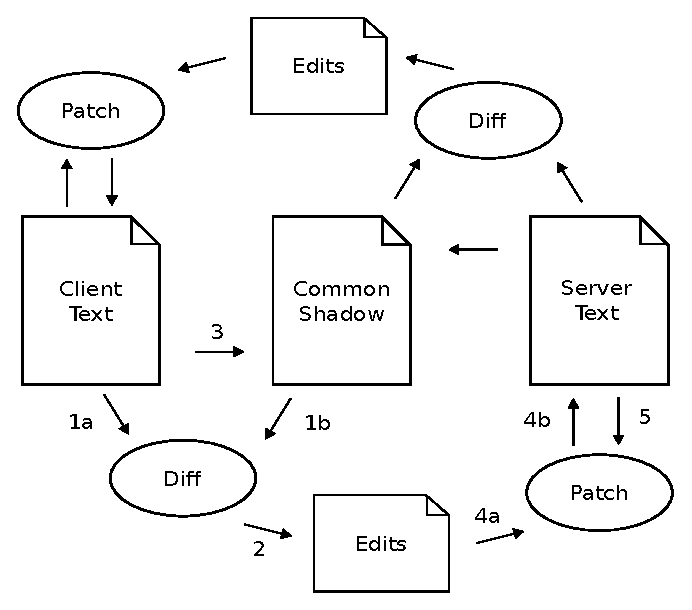
\includegraphics{diff1}
\end{figure}
\par In the beginning Client Text, Server Text and Common Shadow are the same. Client Text and Server Text represent two sides of the collaboration. The goal is to keep them updated. The client and server are allowed to make changes in their documents at any time.
After a specified time interval (timeout), a snapshot of Client Text is taken and using a diff algorithm the difference between the client snapshot and Common Shadow is acquired. Common Shadow represents the last common document state before any edits have been made. The output of this algorithm is a list of changes that have been done by the client. The client snapshot is copied over to the Common Shadow and the changes are patched on the Server Text. Now the process repeats symmetrically using the server text in order to apply changes made by the server or other clients on the client text. This time the Common Shadow is the same as the client snapshot, so diff algorithm returns changes made by the server. The technique is very simple, it is obvious that the main parts of this technique are the diff and patch algorithms.
\par This example is suitable for explanation of the theory behind this technique, but not for use in practice. The problem is that the shadow is common and there is no method to implement this in real life. The client and server must have separate copies of the "Common" Shadow. These copies are called Client Shadow and Server Shadow.
\par We have to make sure that Client Shadow and Server shadow are the same after every synchronization. The delivery is not guaranteed and there is a possibility that the shadows may be out of sync. Neil Fraser in \cite{Fraser} suggests sending a checksum of the shadow together with the list of edits. After these edits are applied, a checksum of local shadow is computed and compared to the received checksum. If they do not match, one of the sides has to send the whole document to get the shadows back in sync. This solution is able to detect the problem with packet loss, but it is not able to solve it without data loss.
\par Differential synchronization has an architecture that enables recovery from this failure. Figure~\ref{fig:ds2} shows this architecture.
\par The main difference is that in this architecture, the server has another shadow text called Backup Shadow to maintain the last version of Server Shadow and both the client and server maintain list of edits that were sent and not acknowledged; in \cite{Fraser} this list is called "outbound stack". Also, the versions of Client Shadow and Server Shadow are labeled with version numbers to be able to detect a failure in communication and acknowledge messages.
\begin{figure}[H]
\caption{DS - Guaranteed Delivery Method \cite{Fraser}}
\label{fig:ds2}
\centering
\vspace{5mm}
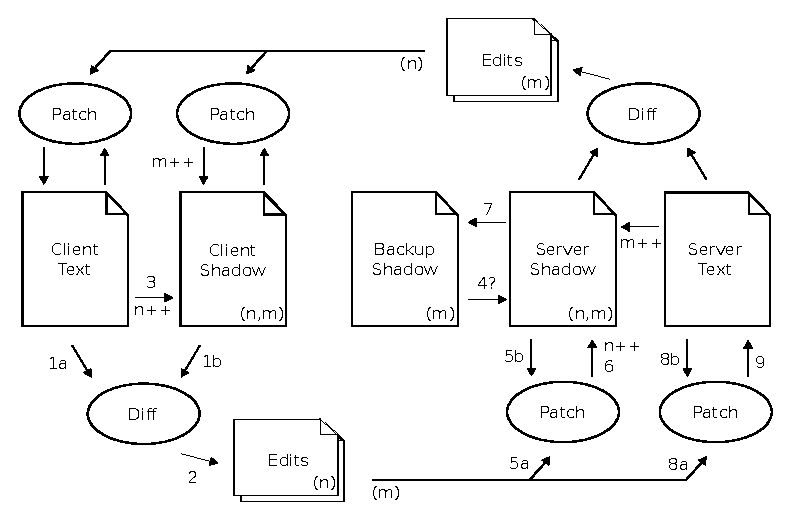
\includegraphics{diff2}
\end{figure}
\par The basic scenario, that is presented in the Figure~\ref{fig:ds2} can be described as follows:
\begin{enumerate}
\item Client text and Client Shadow are used as arguments for the diff algorithm.
\item A list of edits is produced and labeled with the Client Shadow version \(n\).
\item The Client Text is copied to Client Shadow and its version number is incremented.
\item This step is used only in specific situations that are described later
\item A list of edits together with the last known Server Shadow version number \(m\) is sent to the server. This list of edits and the current Server Shadow are used as arguments for the patch algorithm. 
\item The server patches edits to its shadow and increments the last known client shadow version number.
\item The server takes a backup of the current server shadow by copying it in the Backup Shadow. The Backup shadow also contains \(m\).
\item The list of edits and the Server Text are used as arguments for the patch algorithm.
\item The output of the patch algorithm is used to patch the Server Text.
\end{enumerate}
\par The process once again repeats symmetrically; the only exception is that the client doesn't take a backup of his shadow. Every time one of the sites receives an acknowledgement of its edits (\(m\) or \(n\)), it can delete these edits from the outbound stack.
\par This was a description of a normal scenario without failures. To prove that this new architecture is more robust, some other scenarios are described in the following section.
\begin{itemize}
\item \textbf{Lost data sent from a client} - The list of edits sent from the client to the server is not acknowledged. The client keeps all edits in the stack and after the timeout, the client sends new edits together with these old not-acknowledged edits. This repeats until the server acknowledges that some data has been received.
\item \textbf{Lost data sent from the server} - The server sends a list of its edits together with an acknowledgement of the client's last edits. The packet never reaches the client. The client sends some new edits together with the old edits (because the "old" edits were never acknowledged and also never deleted from outbound stack of the client). The server spots that the version number \(m\) received from the client doesn't match version number \(m\) on the server, but it matches \(m\) in the Backup Shadow. It copies the backup shadow to the server shadow (step 4 from basic scenario above). It then applies the new edits received from client and computes a new diff for all edits made by the server and never acknowledged by the client and sends it.
\item \textbf{Duplicate packet} - When the server receives two packets from the client with same number \(n\), its edits from the first one are applied and the second one is thrown away and the communication continues as usual.
\item \textbf{Out of order packet} - The combination of scenarios mentioned above is used. One of the lost data scenarios is used followed by the duplicate packet scenario.\cite{Fraser} 
\end{itemize}
\par The last part of this section is dedicated to diff and patch algorithms. 
\par \underline{\smash{The diff algorithm}} has two main roles in this technique. It is used to retrieve the list of edits made by the user and also to save it in a suitable format. The detection of user edits can sometimes be tricky and the problem of semantic diff versus minimal diff arises. Minimal diff is in most cases not suitable for this implementation as there is a possibility that the user's intention will not be preserved. For example, the change of the word 'win' to 'kid' can be described as the replacement of two letters 'w' and 'n' (minimal diff), but also as a replacement of whole word (semantic diff). When one side changes the word 'win' to 'kid' and the other changes the word 'win' to 'won' the result should be either 'kid' or 'won', which are results of semantic diffs, the word should not be 'kod', which is a result of minimal diffs. "An algorithm must be used to expand minimal diffs into semantically meaningful diffs." \cite{Fraser}
\par \underline{\smash{The patch algorithm}} takes the edits produced by the diff algorithm and patches them to the target text. This algorithm has a role of determining where to patch these edits, because the place where the desired word was at the time of the edit could have changed. It has to solve a dilemma as to whether the patch should be applied at the section with the smallest Levenshtein distance \cite{Levenshtein} between two versions of the document, or if it should be applied at the section closest to the original location. "It is probably more correct to apply a patch onto a near-match at the expected location than to a perfect match at the other end of the document."\cite{Fraser}
\par Another important property of the algorithm that needs to be defined in the implementation is the length of the timeout. A short cycle has higher requirements on the network because DS is constantly sending some information over the network. On the other hand, with a long cycle it is necessary to transfer bigger amounts of data and the probability of collision during a patch is higher. Neil Fraser also mentions in his work that with a rising number of clients scalability may become an issue.
\section{Commutative Replicated Data Types (CRDTs)}
\par The third technique discussed in this paper is called Commutative Replicated Data Types. Although \cite{Shapiro-long} describes CRDTs that are used in various situations, for example as implementation of registers, counters, sets, graphs and sequences, as the main source of information for this section serves the first and most detailed work Designing a commutative replicated data type \cite{Shapiro-design} and later updates and improvements \cite{Shapiro-editing} \cite{Shapiro-consistency}. These papers suggest the use of Treedoc for cooperative editing. This data structure is described later in this section. 
\par An interesting property of this technique is that CRDTs converge without any need of a concurrency control algorithm. This is also the reason, why this section deals mainly with the architecture of the data type and not with the technique as a whole like in the previous sections. Many papers deal with this datatype and highlight its suitability for cooperative editing. Authors in \cite{CRDT-real} evaluated CRDTs for real-time collaboration and found out that this approach is suitable for real-time collaboration. In fact, the paper says that they are better in some aspects than other algorithms. This approach is used in the WOOT \cite{WOOT} and Logoot \cite{Logoot} collaboration systems. Algorithms used in WOOT and Logoot together with RGAs \cite{RGA} are briefly described at the end of this section.
\par "A Commutative Replicated Data Type (CRDT) is a data type where all concurrent operations commute with one another." \cite{Shapiro-design} Operations commute when two sites that started in a same state apply the operations in a different order and the resulting state is also the same. Achieving this property is equivalent to achieving the convergence.
\par This approach also assumes the replication of the document on all sides of the collaboration and unlike the first two techniques this one doesn't use a client-server model in its implementation and instead it uses peer-to-peer architecture. Although it should not be a problem to use this technique with both alternatives. 
\par The smallest unit that can be inserted or deleted is called an atom. This can be a character but also a larger part of the structure, for example in XML whole tags could be considered as atoms. Supported operations are insert(pos,atom) and delete(atom). 
\begin{itemize}
\item insert(pos,atom) - inserts a new atom at a position in document
\item delete(pos) - deletes an atom at the position 
\end{itemize}
Using these two operations, it is possible to produce all other needed operations. It is also easy to implement transactions using CRDTs. 
\par Every atom has its unique position identifier, called UID. This UID is used as a parameter during the execution of the operations. The properties of UIDs are as follows:
\begin{itemize}
\item The identifier is unique and stays the same for every atom throughout the whole life of the document.
\item A total order of identifiers exists.
\item It is always possible to generate a new identifier between any two identifiers. Generally, for any two identifiers \(A\) and \(B\) such that \(A < B\), we are able to create a new identifier \(C\) such that \(A < C < B\).
\end{itemize}
\par The fundamental principle of this technique is that operations are executed locally and sent over the network to all other peers. There should be no need to preserve the order of the operations. This is due to the commutativity property and the uniqueness of identifiers. This uniqueness also ensures that there is no need to transform operations or provide suitable context because it is clear what atom should be edited.
Authors in \cite{Shapiro-design} point out that real numbers are suitable for the role of identifiers, but for implementation it would be necessary to be able to work with infinite precision and that is impossible. The solution suggested in \cite{Shapiro-design} is the use of Treedoc. Algorithms using CRDTs differ mostly in the way of generating/maintaining these identifiers. Figure~\ref{fig:treedoc} shows an example of Treedoc.
\begin{figure}[H]
\caption{Treedoc}
\label{fig:treedoc}
\centering
\vspace{5mm}
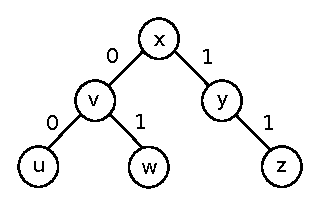
\includegraphics{treedoc1} 
\end{figure}
\par Treedoc is an abstract data structure that is used in document editing. It is implemented as a binary tree and every node represents an atom in the structure. The UID is the path in the tree that starts in the root. Root's UID is an empty string [].
\par Treedoc in Figure~\ref{fig:treedoc} encodes the string 'uvwxyz' and uses characters as atoms. The UIDs for the characters are: u = [00], v = [0], w = [01], x = [], y = [1],z =[11]. This structure ensures the property where it is always possible to generate a new identifier between two existing UIDs. 
\par In the end, the whole document consists of pairs (UID,atom). These are ordered by UIDs. A partial order definition on the identifiers can be found in \cite{Shapiro-design} and also in \cite{Shapiro-editing}. 
\par The delete operation is easy to implement. Deleting is simply replacing the atom in the node with null. If the deleted atom was a leaf it can be completely removed from the memory, and if it was an inner node it is kept in memory and garbage-collected at some point in future. However, the leaf can be completely deleted only when the delete operation is stable, which according to \cite{Shapiro-design}, means that it has been executed on all sides of the collaboration. This paper also introduces a new procedure gc(N) which removes leaf N if it is stably deleted. This operation is executed only locally.
\par The insert operation is harder to implement. The basic algorithm implementing this operation is not trying to keep the tree balanced. This is resolved later by other suitable solutions. The full code of the algorithm can be seen in \cite{Shapiro-design} and \cite{Shapiro-editing}. 
\par Inserting a new atom between two other atoms(atom\(_a\) and atom\(_b\)) is more complicated. First, the algorithm has to check if there is some atom between the supplied atoms. The reason for this is that the algorithm has to insert new a atom between the two already present atoms that have nothing between them. During  the next step, the algorithm figures out whether one of the atoms is an ancestor of the other and there can be 3 different situations:
\begin{itemize}
\item atom\(_a\) is an ancestor of atom\(_b\): In this situation, atom\(_b\) has no left child so this new atom will be the new left child of atom\(_b\). The new UID will be \(uid(b) \cdot 0\)
\item atom\(_b\) is an ancestor of atom\(_a\): In this situation, atom\(_a\) has no right child so this new atom will be the new right child of atom\(_a\). The new UID will be \(uid(a) \cdot 1\)
\item Atoms do not have an ancestry relation:  In this situation, atom\(_a\) has no right child so this new atom will be the new right child of atom\(_a\). The new UID will be \(uid(a) \cdot 1\)
\end{itemize}
\par The ancestry relation is defined as expected. Node \(a\) is the ancestor of node \(b\) if there is \(a\) on the path from \(b\) to the root node. This also means that \( uid(b) = uid(a) \cdot (0,1)^k \) where \(k\) is the difference between the depths of these two nodes.
\par The problem with concurrent inserts is resolved with an extension of the nodes with disambiguators. These disambiguators are pairs of \(idX = (siteID, counter)\) where \(siteID\) represents the site that initiated the creation of this disambiguator and the \(counter\) variable represents the counter that is maintained by each site. There is also a total order of disambiguators defined: \begin{center} \( (s_1,c_1) < (s_2,c_2) \quad iff \quad c_1<c_2 \vee (c_1=c_2 \wedge s_1 < s_2) \) \end{center} This ensures that every disambiguator is unique and that the order of disambiguators is the same on every site. 
\begin{figure}[H]
\caption{Treedoc}
\label{fig:treedoc2}
\centering
\vspace{5mm}
\includegraphics{treedoc2} 
\end{figure}
\par Figure~\ref{fig:treedoc2} shows the use of disambiguators. As this concurrency can occur at every node, authors in \cite{Shapiro-design} suggest the use of disambiguators on every node when it is created and garbage-collecting these disambiguators periodically. An insert operation is stable at some site, when this site receives all operations that happened after this operation has been executed locally. At this point it is clear that there will be no other concurrent inserts. 
\par The last operations designed for this abstract data structure are \textit{explode(string)} and \textit{flatten(path)}. The operation \textit{explode(string)} accepts a string of atoms and returns a tree that is constructed from the supplied string and the operation \textit{flatten(path)} accepts a path from the sub-tree and returns a string of atoms. The flatten operation skips the null nodes on the path. These nodes were produced by deleting inner nodes. The sequential application (\textit{explode(flatten(treedoc)}) of these two operations on an unbalanced treedoc with null nodes results in a new treedoc that has the same content, but it is balanced and without null nodes in the structure. These operations don't commute with the edit operations on the tree. The \textit{explode} operation is not really necessary it can be substituted with applying a path to a string. There is no need to search for a solution for its commutativity. The commutativity of \textit{flatten} operation is ensured by voting. This operation cannot be executed when there is another \textit{insert} or \textit{delete} in progress. Therefore all the sites vote whether the \textit{flatten}x operation can be executed. If one of the sites spots an edit operation it votes "No" otherwise it votes "Yes". \textit{Flatten} is executed only if all sites vote "Yes".
\par The interesting thing about CRDTs is that with this approach it is easy to implement transactions. As the operations commute, all that is needed are labels of the beginning and the end of the transaction and a buffer. When a peer executes local transaction all operations received from network are buffered and vice versa. With transaction support it is easy to implement block operations such as copy and paste or search and replace because we can guarantee that during the transaction the state of the document won't change.
\par The last part of this section deals with the Logoot, WOOT and RGA algorithms, which are alternatives to the original algorithm. All of them use the idea of CRDTs. Logoot and WOOT use only 2 operations that were described earlier, RGAs support also update operations. The only difference is in the way of generating the identifiers. 
\par Logoot tries to avoid the use of tombstones which are deleted atoms that had to remain in the structure, but they are not visible (e.g. null nodes in Treedoc). It has a bit more of a complicated structure for the UIDs and it uses whole lines as atoms. Every site has its site identifier \(s\) and a "clock" \(h_s\) that is incremented each time a line is created at particular site. Every line has its position \(pid\) in the document. The position is a list of identifiers and an identifier is a couple of \(<p,s>\) where \(p\) is an integer and \(s\) is the unique site identifier. The whole document consists of pairs \((pid,text)\). Also, the first and last line are uniquely identified by having \(l_B\) (beginning) and \(l_E\) (end) in the text variable. An example line generated by site \(s\) can look like this: \( ((<i,s>,h_s),text) \). New UIDs are generated by adding more identifiers (\(<i,s>\)) in the first part of the position tuple and by updating \(h_s\). The order of the identifiers can be described as lexicographic. Authors of Logoot point out that the use of tombstones generates a big overhead, so they tried to avoid it by using new format of identifiers. More information can be found in \cite{Logoot}.
\par WOOT was one of the first algorithms that used CRDTs. The time complexity is not as good as Logoot's time complexity; this is caused mainly by the use of thombstones. WOOT identifies characters as atoms and every character has a unique identifier; these atoms are called W-characters. This W-character is a tuple \( <id,\alpha,v,id_{cp},id_{cn}> \) where \(id\) is the identifier of the character which is a couple constructed of a unique identification number of the site and a logical clock. \(\alpha\) is the actual value of the character. \(v\) is a boolean value that represents visibility and \( id_{cp}, id_{cn} \) are identifiers of the previous and next character. These identifiers are the reason why there have to be tombstones. They are necessary to identify the exact position of the character on each site. Partial order between the atoms is defined and the uniqueness of the UIDs is ensured by a unique identifier of the site and with the logical clock. The supported operations are also insert and delete. 
\par RGAs are the third major algorithm used for implementation of CRDTs. This algorithm seems to be the most complicated one from all presented alternatives but achieves the best results. These results are achieved with the use of hash tables; this detail reduces the time necessary for finding the correct place for operation.  It uses Replicated Growable Arrays and supports not only insert and delete operations, but also an update operation. These RGAs are built from RFA (Replicated Fixed Arrays) and RHT (Replicated Hash Tables). This approach also uses tombstones, but tries to remove them, when they are not needed. RGAs maintain a liked list of elements and a local operation finds the correct place using simple integer indexes. Remote operations find the correct place via hash tables and with unique indexes. More detailed information about this approach and about all data structures mentioned in this paragraph can be seen in \cite{RGA}. This paper also defines s4vector as the unique identifier that consists of four elements. S4vector is a tuple \(<a,b,c,d>\) where \(a\) is a global session number, \(b\) is a unique site identifier, \(c\) is the sum of the vector clock \(v[]\) and \(d\) is reserved for purging tombstones. 
\chapter{Comparison of Techniques}
This chapter presents a comparison of these techniques using the criteria described in the following section. The chapter belongs to the theoretical part of the thesis, so the comparison is more general. 
\section{Comparison Criteria} \label{comparison}
This section describes the comparison criteria for the presented techniques and presents the reasons for choosing these particular criteria. These criteria, together with other requirements, are used in section \ref{requirements} for describing the Komodo requirements for real-time collaboration and in section \ref{best} for choosing the best technique.
\par The comparison criteria include:
\begin{itemize}
\item client-server vs. peer-to-peer model,
\item requirements on a local machine vs. a remote machine,
\item amount of data transfer,
\item network requirements,
\item time complexity,
\item conflict resolution ability,
\item latency tolerance,
\item and supported content formats.
\end{itemize}
\par It is important to determine whether the technique can be used only with the client-server model or with the peer-to-peer model or with both of them. Also related with this requirement is the scalability of the technique, how many users could participate in the collaboration. This is important for use in practice because this can be one of the most fundamental requirements of the system. When evaluating architecture criterion, we assume that the number of collaboration sites is greater than two.
\par One of the comparison criteria is performance requirements. These requirements should be reviewed as requirements on a local machine vs. requirements on a remote machine. Some techniques might have tougher requirements on the client side and other on the server side. The evaluation of these requirements is also dependent on the architecture.
\par The amount of data transfer is also important. The more data that it is necessary to transfer the harder it is to implement this technique in environments with collaboration sites in distinct parts of the world. The best practice is to transfer the least amount of data as possible. This criterion should be reviewed in contrast with other techniques.
\par The network requirements should be taken into account because it is necessary to know if one of the techniques requires a particular protocol or some other network functionality. Some of the techniques may not be suitable for bigger networks like the Internet.
\par Time complexity is very closely related to the requirements placed on the machines. This criterion focuses on the time complexity of the algorithms that ensure consistency maintenance. Some of the techniques might do the majority of the work in the algorithm while others may have done some preparation and the following algorithm is not so complex.
\par The conflict resolution ability is also assessed. The main goal is to have as few conflicts as possible, but when some conflict occurs, it is necessary to resolve it as quickly as possible and with the correct result. All of the techniques are able to resolve conflicts, but the important part is the correctness of the result. 
\par The best technique should also be able to tolerate the latency of the network. The ability to recover from a lost packet situation or to recover from a situation when the packets come out of order is also important. 
\par The last criterion is ability to process various content formats. This part should point out which formats are supported and which are not supported by a particular technique.
\section{Comparison}
\par This section evaluates the techniques according to the presented criteria. The main part is divided into the different techniques which are evaluated according to each criterion. In the last part of the comparison a table  is presented to summarize the findings of this section.
\\
\par \textbf{\underline{\smash{Operational Transformation}}}

\vspace{3mm}

\textbf{Client-server vs. peer-to-peer model} - Majority of articles about Operational Transformation used in this thesis suggest the client-server model for this technique. The main reason why this technique cannot be implemented with a peer-to-peer model is the fact that the client has to send operations that come from a state in the server's history. This would imply that every peer would have to preserve the history of every other peer to be able to send such operations. This problem already occurred in the design of Operational Transformation, and was resolved by moving the responsibility to track the history from the server to clients.

\vspace{3mm}

\textbf{Requirements local vs. remote} - In this technique, the requirements on the local machine are slightly higher than on the remote server. As mentioned above, the client has to track the server's history and send only particular types of operations. The server solves only the diamond problem and sends out operations that it receives.

\vspace{3mm}

\textbf{Amount of data transfer} - Operational Transformation only sends operations over the network. New algorithms for implementation of this technique also send parenting information and other implementations could have more metadata, but this metadata should not enlarge the packets significantly. It is necessary to transfer the whole document only in network failures. The amount of data transfer necessary for this technique is low.

\vspace{3mm}

\textbf{Network requirements} - This technique assumes the use of a connection over TCP protocol \cite{Jupiter}\cite{simplified} in order to ensure the delivery. However, the mechanism should be able to detect lost packets, because the server has to acknowledge operations that the client sends. 

\vspace{3mm}

\textbf{Time complexity} - The Time complexity for consistency maintenance is linear.\cite{sequence}\cite{orthogonal} For other more specific and more difficult functions, like undo the complexity can be non-linear.

\vspace{3mm}

\textbf{Conflict resolution ability} - The transformation function is the main part that ensures good conflict resolution. The role of this function is to transform the operations against each other in order to preserve the user's intention, convergence and causality.

\vspace{3mm}

\textbf{Latency tolerance} - As was mentioned above, the server has to acknowledge user operations. Acknowledgement serves mainly for the client to know server state, but can also be used for latency tolerance. This means that the chance that user operations will get lost is very small. It also implies that the server preserves a version of the document on which all operations were applied. In case of inconsistency, the whole document can be transferred to the user.

\vspace{3mm}
\newpage
\textbf{Supported content formats} - Operational Transformation is able to process plain text, but also a variety of other formats like XML and other tree structured data types. This technique is used also in graphics editing systems \cite{graphics} like CoFlash and also for collaborative slides creation and presentation in CoPowerPoint.

\vspace{3mm}

\par \textbf{\underline{\smash{Differential Synchronization}}}

\vspace{3mm}

\textbf{Client-server vs. peer-to-peer model} - This technique is also not suitable for a peer-to-peer model. It would be really computationally complex for each client to maintain \((n-1)\) peer shadows and to compute \((n-1)\) diffs and the patching would be really hard. With a rising number of peers the real-time collaboration would be impossible to implement.

\vspace{3mm}

\textbf{Requirements local vs. remote} - Differential Synchronization has harder requirements on the server than on the client. Neil Fraser \cite{Fraser} points out that the algorithm is symmetrical, which means that an (nearly) identical code is running on all machines. However the final version of the algorithm presented in his paper is more difficult for the server. It has to maintain another shadow for the case of data loss and the server is also responsible for broadcasting the operations to every client and for patching all operations on its document version. It is also necessary that the added shadow maintained for every client.

\vspace{3mm}

\textbf{Amount of data transfer} - Data transfer might be the highest among these techniques because the changes made in a document described in a diff file are provided with context. The context must be large enough in order to find the right place for patching.

\vspace{3mm}

\textbf{Network requirements} - No special properties of the network are necessary for this technique. Differential synchronization has a good mechanism that is able to recover from a loss of packet.

\vspace{3mm}

\textbf{Time complexity} - The Time complexity depends on the diff and patch algorithms and can differ with the content format and with the choice of these algorithms, as there can be more algorithms for the particular content format. For example, one of the diff algorithms for XML files is XyDiff\cite{Xdiff} and this algorithm achieves \(O(nlogn)\) complexity in the execution time.

\vspace{3mm}

\textbf{Conflict resolution ability} - This property depends on the patch algorithm. One of the roles of this algorithm is to identify the conflict and to be able to resolve it with the correct result. The choice of the algorithm is free so it can not be evaluated in general.

\vspace{3mm}

\textbf{Latency tolerance} - There is a good guaranteed delivery method used in this technique that is described in the previous chapter. Almost every situation can be resolved without having to send the whole document over the network.

\vspace{3mm}

\textbf{Supported content formats} - Differential synchronization can be used with every format as long as there are diff and patch algorithms for the desired format present.

\vspace{3mm} 

\par \textbf{\underline{\smash{Commutative Replicated Data Types}}}

\vspace{3mm} 

\textbf{Client-server vs. peer-to-peer model} - Peer-to-peer architecture is presented in most cases for this approach. Sites of collaboration only send the operations that have been completed locally so there is an option to broadcast the operations to every peer and also to send operations to one server that will take care of broadcasting operations to the other clients.

\vspace{3mm} 

\textbf{Requirements local vs. remote} - Requirements are equal on each site of the collaboration. Every site has to maintain the correct order of identifiers and send\textbackslash receive operations. This also depends on the architecture. If a client-server model is chosen, the requirements on server would be higher because the server would have to broadcast the messages.

\vspace{3mm} 

\textbf{Amount of data transfer} - The amount of data transfer in this approach is comparable to the amount needed in Operational Transformation. The atoms of the document are uniquely identified, so there is no need to provide context. Only the operations and the identifier of the atom are sent over the network.

\vspace{3mm} 

\textbf{Network requirements} - There are no special requirements of CRDTs for the network. One of the reasons could be that this technique is concerned mainly with the identification of the atoms and doesn't concern itself with the network problems, such as packet loss or packets that are out of order.

\vspace{3mm} 

\textbf{Time complexity} - The Time complexity is dependent on the chosen type of identifiers and on the algorithm that generates new identifiers. The technique itself only sends operations over the network. The key point is the ability of the algorithm to generate a new identifier or to find the correct place for the insertion of a new atom. It can not be evaluated in general as it was by Differential Synchronization. For example, according to \cite{CRDT-real} WOOT has a worst-case time complexity of the insert operation equal to \(O(n^3)\) and the time complexity of delete is equal to \(O(n)\) where \(n\) is the number of atoms. Time complexity information for other algorithms can also be found in \cite{CRDT-real}.

\vspace{3mm} 

\textbf{Conflict resolution ability} - Every atom is uniquely identified so there should be no conflict. Where there are two concurrent operations that try to delete the same atom, the second delete operation will find a tombstone and assume that is has been already deleted. The concurrency of two insert operations at the same place is resolved individually by each algorithm that generates identifiers.

\vspace{3mm} 
\newpage
\textbf{Latency tolerance} - As it is mentioned above, this technique deals mainly with the identification of atoms, so the mechanism for latency tolerance is very weak. Every site basically logs its operations (both local and remote). A new site or crashed site will receive the whole document and a site that was disconnected for a while receives all missing operations.\cite{Shapiro-design}

\vspace{3mm} 

\textbf{Supported content formats} - This technique can also support any format of content. The fundamental element is the division of the content to atoms and their identification. The interesting property of this approach is that a bigger part of the document can be considered as an atom, for example whole XML tags.

\vspace{13mm} 
\newpage
\noindent
\begin{tabular}{| p{1.7cm} | p{2.2cm} | p{2.2cm} | p{2.2cm} | p{2.2cm} |}
\hline
 & C-S vs. p2p & local vs. remote* & data \newline transfer & network req.  \\
\hline
OT & C-S & local & low & use of TCP assumed \\
\hline
DS & C-S & remote & higher & no special \\
\hline
CRDTs & both & equal & low & no special \\
\hline
\end{tabular}
\newline
\vspace*{1 cm}
\newline
\begin{tabular}{| p{1.7cm} | p{2.2cm} | p{2.2cm} | p{2.2cm} | p{2.2cm} |}
\hline
 & time** \newline complexity & conflict resolution*** & latency tolerance  mechanism & content formats \\
\hline
OT &  \(O(n)\) & X & average  & any \\
\hline
DS & \(O(nlogn)\) & X & strong  & any \\
\hline
CRDTs & \(O(n^3), O(n)\) & X & weak  & any \\
\hline
\end{tabular}
\vspace{10mm}
\newline
* The table describes on which site the requirements are higher. \newline
** With all techniques, time complexity is dependent on implementation; time complexities are only informative. \newline
*** Conflict resolution ability cannot be compared in this table. In each case this ability depends on the choice of a particular function/algorithm.
\chapter{Red Hat JBoss Data Virtualization}
\par This chapter covers the practical part of the thesis; it briefly describes the Red Hat JBoss Data Virtualization platform, an Eclipse-based design tooling called Teiid Designer and its new upcoming version Komodo. In the next section, the requirements of Komodo for real-time collaboration are presented and the following part deals with choosing the best technique for Komodo from the three presented techniques in the theoretical part. The last part deals with the Java implementation of this technique that can be used in the actual implementation of real-time collaboration in Komodo.
\section{Overview}
\par The Red Hat JBoss Data Virtualization platform is a product based on a community project called Teiid.  This software is able to federate and integrate data sources of all kinds like SQL data sources, non-SQL databases, Flat files, XML files, Excel files, web services and more. It makes the development of new applications easier because the software developer doesn't have to query every data source needed by the new application and federation of the data in the application is not necessary. The Data Virtualization platform will do this for the developer. It has a set of translators that are able to "translate" the content from various formats to Teiid server logic.
\par This platform is able to create one virtual database called VDB that will federate all underlying data sources and make it look like there is only one data source. User can also use a security mechanism that is able to limit  access only for certain users and many other features. Data Virtualization runs on top of the application server called Red Hat JBoss Enterprise Application Platform. Figure~\ref{fig:dv} shows the architecture of Red Hat JBoss Data Virtualization platform.
\begin{figure}[H]
\caption{Red Hat JBoss Data Virtualization\cite{dvimage}}
\label{fig:dv}
\centering
\vspace{5mm}
\includegraphics[scale=0.65]{dv} 
\end{figure}
\par Users of this product are able to create VDBs in two ways. One is to manually create an XML file with a certain structure. This VDB is called Dynamic VDB. In this VDB, the user describes what data source defined on server they want to use and the user can specify all the needed information for the federation of the data sources. 
\par Another alternative is to create a project in Teiid Designer. Teiid Designer is an Eclipse-based designing tool for Data Virtualization. It is much easier to create connections to remote and local data sources and also to federate them using this tool. The user imports metadata from various data sources. These metadata about a data source are represented in Teiid Designer by a Source model. The user can specify which tables, columns or other types of structure they want to include in their project. There are also View models present in which the user can specify the federation schema and alter the structure of the tables provided by the Source model. We can say that the Source model represents the physical data storage and the View model represents a business view of the data. In the end, the models are included in a static VDB file. Static VDBs are basically ZIP packages containing XML models and other information, they are more complicated and not easy to create without tooling. 
\par These VDBs are then deployed to the Teiid server and external users/applications can query this new database. This VDB acts as one SQL database and doesn't expose the internal structure. The user can also choose to produce a web service instead of a VDB. 
\par Another benefit of Red Hat JBoss Data Virtualization is also the fact that it enables querying data sources that are not easy to query without Data Virtualization. These data sources are for example Flat files, XML files and Excel spreadsheets.
\section{Komodo}
\par This section should provide some basic information about Komodo and the differences and improvements that will be included in Komodo. All information about Komodo that is presented in this section is from members of the Komodo developing team or from the Komodo Release Development plan \cite{Komodo}. 
\par Komodo should be a new version of Teiid Designer which has many new features and tries to get the designing tool closer to the Teiid server. The main impulses for creating a new tool for Data Virtualization come from changes in Teiid 8.x and the use of dynamic VDBs in the Openshift platform.  
\par The fundamental difference in the architecture of this tool is the division into two parts, the KEngine and User Interface (UI). The KEngine will be the main part that will handle all necessary functionality and will form the core of the application. This engine should adapt the common Teiid DDL dialect for relational data definition. KEngine will have Command Line Interface (CLI) through which all activities will be possible to perform. The user will be able to choose between CLI and UI.
\par The CLI is being finalized at the time of the writing this thesis. The user will be able to create models and VDBs using a few simple and understandable commands like CREATE, RENAME, DELETE, SET and others.
\par The User Interface will provide a clickable interface for users and to this day it has not been decided if the UI will be web-based or Eclipse-based. New UI should not include the Eclipse modeling framework used in Teiid Designer.
\par Another change in Komodo is the use of ModeShape as a place for storing information about models and VDBs. Komodo won't use Eclipse workspace anymore. It should use KSpace which will be a new workspace that is based on JCR, e.g. ModeShape. 
\par "ModeShape is a distributed, hierarchical, transactional, and consistent data store with support for queries, full-text search, events, versioning, references, and flexible and dynamic schemas."\cite{ModeShape} It implements the JSR-283\footnote{\url{https://jcp.org/en/jsr/detail?id=283}} standard Java API from content repositories also known as JCR. This kind of repository is a suitable solution for Komodo because it is good at storing hierarchical data, file storage, and also at versioning and many other aspects. 
\par Data in ModeShape are stored in a form of nodes connected to each other.  ModeShape has some basic node types already defined, but in most cases it is necessary to define custom nodes for the desired application. This definition of node types is called Compact Node Definition. Komodo nodes in the repository will be Teiid Dynamic Artifacts. These artifacts are for example models, tables, columns, DDL statements, and so on. Komodo has already prepared the majority of these definitions\footnote{\url{https://raw.githubusercontent.com/Teiid-Designer/komodo/master/plugins/org.komodo.modeshape.teiid.sql.sequencer/cnd-examples/StandardDdl.cnd}}\footnote{\url{https://raw.githubusercontent.com/Teiid-Designer/komodo/master/plugins/org.komodo.modeshape.teiid.sql.sequencer/demigen/org/komodo/modeshape/teiid/cnd/TeiidSql.cnd}}. There is also a suggestion to use multiple local KSpaces and also remote KSpaces for collaboration purposes. 
\par One of major changes in approach of the modeling in this new tool, is that the creation of a new VDB should be "VDB-centrinc" instead of "Project-centric". In other words the creation of a VDB in Teiid Designer begins with creating a Model Project, as a next step user creates models and then they include these models in a VDB which is deployed to the server. Komodo won't use Projects. The user will create an artifact and then it can be saved in a local library for later use. The workspace concept contains VDBs and/or models.\\ \\
The major conceptual changes are summarized in six points\cite{Komodo}:
\begin{enumerate}
\item \textbf{Simplify terminology} - Terminology of Teiid Designer is sightly different from the terminology used by Teiid. Komodo should eliminate these differences.
\item \textbf{Replace the notion of "Source models" with "Data sources" }- This point is in strong relation with the first one. It is more understandable to name the base models as Data Sources as this terminology is also used by the Teiid server.
\item \textbf{Expose Create Views or Virtual Procedures as a primary feature} - There is an effort to remove the diversity of models, Teiid Designer has a lot of model types such as Source, View, Relational, Web Service, XML and other. The number of models should be cut down and the user will use simpler DDL constructions.
\item \textbf{Expand the notion of a VDB in the workspace} - Komodo will implement Teiid's Dynamic VDB functionality.
\item \textbf{Ability to connect to multiple KSpaces} - Komodo will add an ability to have multiple local or remote workspaces as was already mentioned above.
\item \textbf{New global workspace location concept} - Standard Eclipse workspace has many drawbacks. For example, when users switch workspaces, the connection profiles have to be exported from the old workspace and reimported into the new one. A global workspace should store these common data outside of a regular workspace.
\end{enumerate}
\section{Komodo Requirements for Real-time Collaboration} \label{requirements}
\par This section describes the requirements on real-time collaboration that are set by Komodo software. All information presented in this section also come from the Komodo Release Development plan \cite{Komodo} or from conversations with the development team.

\vspace{3mm} 

\textbf{Architecture model} - Komodo is able to use the client-server model in its implementation of the real-time collaboration. This approach seems to be more suitable for real-time collaboration. This is in relation with the requirement for the number of collaboration sites.

\vspace{3mm} 

\textbf{Remote vs. local requirements} - There is no specification on which side the requirements should be greater. The server will have to broadcast the changes and maintain a server version of the document which means it will have to receive changes from a number of clients. On the other hand, the client deals with the actual modeling of the artifact and with sending and receiving messages.

\vspace{3mm} 

\textbf{Amount of data transfer} - Obviously, the amount of data transfer should be as small as possible. In order to make the technique as fast as possible. The VDB files are as small as they can be because they don't hold any data and store only DDLs for transformation of data into the desired format.

\vspace{3mm} 

\textbf{Network requirements} - Komodo doesn't have any special network requirements. The only requirement is that real-time collaboration should be implemented over the Internet.

\vspace{3mm} 

\textbf{Latency tolerance} - As the real-time collaboration should be performed over the Internet, latency tolerance should be as good as possible.

\vspace{3mm} 

\textbf{Data type} - Although Komodo will use ModeShape for data storage, real-time collaboration should deal with dynamic VDBs. These VDBs are in the form of XML files as was mentioned previously. The structure of an example VDB XML file can be seen in the Komodo Release Development plan\cite{Komodo}. It consists mostly of a few XML tags and DDL statements. This content format requirement is very important and has the main impact on the choice of the technique.

\vspace{3mm} 

\textbf{Number of participants} - The number of users collaborating on one model/vdb/artifact can be greater than two. The client-server model should be more suitable for the rising number of users. The chosen technique should be well scalable.

\vspace{3mm} 

\par Aspects of Time Complexity and the Conflict Resolution ability are not mentioned because it is obvious that these two properties should be as good as possible.
\section{The Best Technique for Komodo} \label{best}
\par This section deals with choosing the best technique for Komodo from the three presented techniques and according to the requirements set out in the previous section. At the end of the section, a short reasoning is provided as too why we chose CRDTs as the best technique for Komodo. 

\vspace{3mm} 

\textbf{Architecture model} - All three techniques are able to work with the client-server model. This requirement doesn't rule out any of the presented techniques.

\vspace{3mm} 

\textbf{Remote vs. local requirements} - Komodo doesn't have any requirements/limitations in this area. It is not necessary to rule out any of the techniques.

\vspace{3mm} 

\textbf{Amount of data transfer} - Operational Transformation and CRDTs have the lowest data transfer. Although the amount of data transfer in Differential Synchronization is not significantly high it seems to be less suitable for Komodo.	

\vspace{3mm} 

\textbf{Network requirements} - Komodo has no special requirements/limitations for the network. This aspect doesn't rule out any particular technique.

\vspace{3mm} 

\textbf{Latency tolerance} - The best latency tolerance mechanism is presented by Differential Synchronization. The other two techniques do not significantly deal with latency tolerance in the presented papers, although latency tolerance should not be problem in the two remaining techniques.

\vspace{3mm} 

\textbf{Data type} - All of the techniques are able to process any data format. In the case of Differential Synchronization, there should be diff and patch algorithms present for the desired data format. Operational Transformation was implemented for Google Wave and this application worked with Waves as XML files. There are also diff and patch algorithms present for XML files. One of the examples (XyDiff) is referenced in section \ref{comparison}. CRDTs are able to process XML and might be the best solution for Komodo considering this aspect because we can choose what part of the data can be an atom for this technique. Not only whole XML tags can be considered as atoms, but also some main and stable parts of DDL such as CREATE, VIRTUAL PROCEDURE, SELECT, FROM, WHERE etc.

\vspace{3mm} 

\textbf{Number of participants} - This requirement seems to be the breakpoint in deciding which technique is the best for Komodo. As Neil Fraser \cite{Fraser} points out, there can be a scalability problem with the rising number of participants in Differential Synchronization.

\vspace{3mm} 

Commutative Replicated Data Types (CRDTs) were chosen as a the best technique for implementation in Komodo. 
\par The problem with scalability and higher data transfer in comparison with the other two techniques ruled out the Differential Synchronization as the best technique for Komodo. Operational Transformation seems to be a good theoretical technique for real time collaboration, but implementing this technique on a reliable level is hard. Considering real-time collaboration in Komodo, a minor feature and not the main feature of the software, it should not be hard and time-consuming to implement. The Google Wave implementation of Operational Transformation, which is known today as Apache Wave\footnote{\url{https://incubator.apache.org/wave/}}, is an open-source project. It deals with XML files so it could be used in Komodo, but it would not be easy to modify for Komodo because it is big and comlicated. Also authors in \cite{CRDT-real} point out that the only existing transformation function that is reliable is TTF (Tombstone Transformation Function)\cite{ttf} that uses tombstones and does not delete characters immediately. This is not considered as a shortcoming because Treedoc in CRTDs also uses tombstones, but it changes the approach in OT and brings it closer to the idea of CRDTs. Also, according to \cite{CRDT-real}, Logoot and RGA algorithms outperform between 25 to 1000 times faster than the SOCT2 OT algorithm.
\par The positives of CRDTs are: the possibility to define larger parts of the document as atoms, low data transfer, native support of transactions and compatibility with nearly any content type, first of all with XML. 

\section{Java Implementation}
\par This section describes a Java implementation of the chosen technique which is CRDTs. There was no suitable implementation found so this section describe possibilities and requirements for a new implementation of this technique suitable for Komodo. 
\par We haven't found a suitable Java library that would implement CRDTs and that can be used for the collaborative editing of XML files. It appears that such a library is not implemented yet despite the fact that CRDTs were evaluated as a good solution for collaborative editing. In the following paragraphs some open-source projects that use CRDTs are mentioned. 
\par The found implementations of CRDTs include the Database system Riak. This is an open source project that presents itself as a Non-SQL database and works with Riak Data Types\footnote{\url{http://docs.basho.com/riak/2.0.2/dev/using/data-types/}} which are inspired by CRDTs.
\par We have also found some implementations of the WOOT system for collaborative editing in Javascript\footnote{\url{https://bitbucket.org/d6y/woot}} and in CoffeeScript\footnote{\url{https://github.com/kroky/woot}}.
\par With new a implementation comes the possibility to choose an algorithm for generating the identifiers. We can choose from the major algorithms in this area which are: the Treedoc, WOOT, Logoot and RGA algorithms. According to \cite{CRDT-real}, the best overall performances are achieved using the Logoot and RGA algorithms. The WOOTH algorithm, which is the optimization of WOOT, seems to have comparable performance to RGA. In this paper a more detailed comparison of these algorithms can also be found. RGA and WOOTH seem to have a better performance because of the use of hash tables. The Logoot algorithm is designed to use whole lines as atoms, but this can be certainly changed Logoot can be used with characters or other atoms. The literature points out that Logoot identifiers can grow unbounded, but experiments with Wikipedia entries have shown that this problem is only theoretical and does not occur in real implementation \cite{Logoot2}.
\par We propose using the RGA algorithm for the case of better performance and harder implementation, and Logoot or WOOTO, which is an optimized alternative of WOOT, for the case of a slightly worse performance and easier implementation. The decision is left to the Komodo development team.
\par An important requirement is of course the ability to work with XML files, especially with dynamic VDBs.
\par Another recommendation is an already mentioned option to use longer and static parts of text in dynamic VDB files as atoms, e.g. XML tags, and static parts of DDL statements.
\par The last requirement is the implementation of the technique with the client-server model, because this model should be more suitable for Komodo.
\chapter{Conclusion}
\par The main impulse for the creation of this thesis was the interest of Komodo development team in the possibility of the use of real-time collaboration in their new software. Users of the existing modeling tooling would like have the opportunity to collaborate on bigger models and the Komodo team showed interest in extending the basic collaboration to real-time collaboration.
\par The first goal of the thesis was to study the three techniques for real-time collaboration and compare them using the presented parameters. The techniques are explained in the second chapter of this thesis. Articles and technical reports were used as sources of information for this chapter. Differential Synchronization is explained using less literature sources. This is due to the few articles that deal with this topic. The comparison, which is presented in the next chapter, was done using more parameters than was suggested in the description of the thesis. 
\par The second goal was to recommend a suitable technique for Komodo modeling software. The fourth chapter represents the practical part of the thesis and describes Red Hat JBoss Data Virtualization and the existing Eclipse tooling called Teiid Designer. Another section describes Komodo and its requirements for real-time collaboration. In the following section, the best technique for Komodo which is Commutative Replicated Data Types, is presented. Suitable existing Java implementation was not found so the last section describes recommendations and requirements for new implementation in the Java programming language. This section also recommends algorithms for the implementation of this technique, but leaves the choice of the particular algorithm to the Komodo team.
\par We think that all goals set in the description of the thesis were successfully reached.
\par In future work, authors can deal with the actual implementation of this technique for Komodo as well as with its improvements. Another possibility is to investigate deeper the modifications and alternatives of Commutative Replicated Data Types, which are Conflict-free Replicated Data Types and Convergent Replicated Data Types and their suitability for real-time collaboration. Also, there is an option to investigate the possibilities of real-time collaboration on ModeShape nodes, because there is a possibility that Komodo would leave out the XML files from the application and it would use them only to export and import VDBs.
\printbibliography 
\end{document}
